% Crucial Preamble
\documentclass[12pt,letterpaper]{article} \usepackage{amsmath} \usepackage{graphicx} \usepackage[margin=1in]{geometry} \usepackage{longtable}  \usepackage{amssymb}

% Extra Preamble
\usepackage{fancyhdr} \usepackage{enumitem} \usepackage{float} \usepackage{soul}
\usepackage{multicol} \usepackage[compact]{titlesec} \usepackage{listings}


% frames with display breaks
\usepackage{mdframed}
\allowdisplaybreaks

% change spacing
\usepackage{setspace}
\setlength{\parskip}{0.4\baselineskip}

% Remove paragraph indentation
\setlength{\parindent}{0pt}

% Reduce space before and after section headings
%\titlespacing*{\section}{0pt}{0.1\baselineskip}{0.2\baselineskip}

% changes font
%\renewcommand{\familydefault}{\sfdefault}

% adds header and footer
\pagestyle{fancy}
\fancyhead{} \fancyhead[C]{CEG 2136 Cheat Sheet} \fancyhead[L]{CEG2136} \fancyhead[R]{Owen Daigle}
\fancyfoot{} \fancyfoot[C]{\thepage}


\begin{document}
	
	\begin{center}
		\Large\textbf{CEG 2136 Cheat Sheet} \\
		\vspace{0.5em}
	\end{center}
	
		\section{Chapter 1}
		
		This chapter is mostly a review of ITI 1100.
		
		
		\section{Chapter 2}
		
		\subsection{Multifunction Circuits}
		This is a circuit that preforms more than one function. For example, a circuit can store if $S=0$, and count up if $S=1$.
		
		\begin{center}
			\begin{tabular}{|c|c|}
				\hline
				A1A0 & Function \\
				\hline
				00 & Store \\
				\hline
				01 & Count up \\
				\hline
				10 & Load \\
				\hline
				11 & Clear \\
				\hline
			\end{tabular}
		\end{center}
	
		Next we will make a state table with the following columns (assuming we are doing a D flip flop which is easy and 4 bits)
		
		\begin{center}
			\begin{tabular}{|c|c|c|c|}
				\hline
				A1A0 & Q3Q2Q1Q0 & Q3'Q2'Q1'Q0' & D3D2D1D0 \\
				\hline
				\textit{operation} & \textit{current state} & \textit{next state} & \textit{flip flop inputs} \\
				\hline
			\end{tabular}
		\end{center}
	
		Then we can create all 4 flip flops, and then put a MUX in front of each of them with the correct operations (with A1A0 as selectors)
		
		\begin{mdframed}[]
		\textbf{Ex. Design a multifunction register as specified in the table using T flip flops.}
		\begin{center}
		\begin{tabular}{|c|c|c|}
			\hline
			\textbf{c1} & \textbf{c0} & \textbf{Function} \\
			\hline
			0 & 0 & Store registers contents \\
			\hline
			0 & 1 & Left Shift (serial input connected to input I) \\
			\hline
			1 & 0 & Count Down \\
			\hline
		\end{tabular} 
		\end{center}
	
		\textbf{Store: } The store is easy, since T ff, we just feed in 0.
		
		\textbf{Left Shift} We are not sure about this one. It would be easy with a D ff, but we are using a T. Whenever we are unsure, we create a table to visualize it. 
		
		\begin{center}
		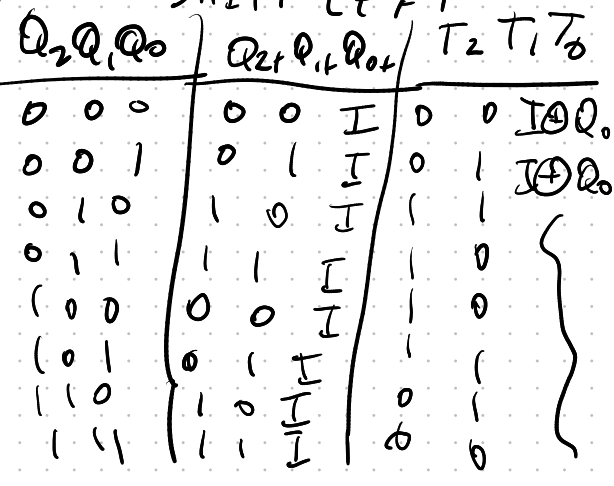
\includegraphics[width=0.5\linewidth]{ex1}
		\end{center}
	
		For the T2 and T1, it is self explanatory. For T0, we need the XOR because again we are using T ffs not D ffs. It makes sense, just trust me. 
		
		Now for the T2 and T1, we need an equation so use 2 k maps to get:
		\begin{align*}
			T_1 = Q_1 \oplus Q_2 \\
			T_2 = Q_2 \oplus Q_1 \\
			T_0 = I\oplus Q_0
		\end{align*}
	
		YAY!! Now we just need 1 more ops. 
		
		\textbf{Count Down: } This is the same process as the shift left. We just need to create the state table, and then find the values for T2T1T0 using K maps: 
		\begin{align*}
			T_0 = 1\\
			T_1 = Q_0 '\\
			T_2 = Q_1 ' Q_0 '
		\end{align*}
	
		Now we are done. We know how to do each of the 3 operations, we just need to \emph{choose} between them. Since we see \textbf{choose}, we know MUX.
		
		We can ignore the last input of our 4x1 muxs since we do not need it. 
		
		\begin{center}
		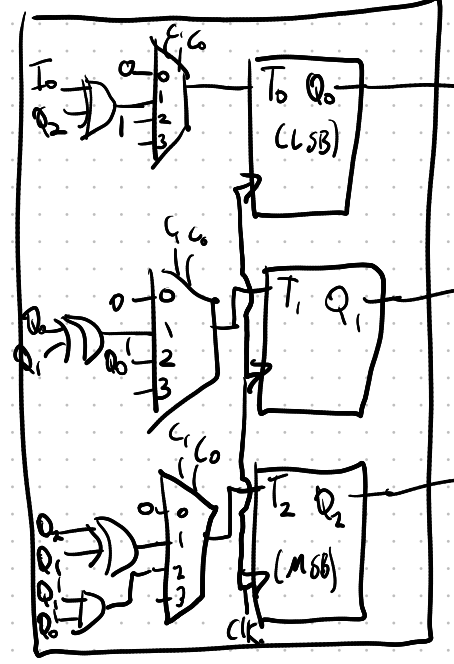
\includegraphics[width=0.5\linewidth]{ex2}
		\end{center}
		
		Most cases are not this bad since we use D flip flops. 
		
		For example, for the left shift using a D, we just put D2 as D1, and D1 as D0, and then D0 as I. SIMPLE!!
		\end{mdframed}
		
		\subsection{Memory}
		If we have $k$ address lines in a memory chip and $n$ data output lines, it means we can store $2^k$ $n$ bit words in that memory chip.
		
		
		\section{Chapter 3}
		\subsection{2s Compliment in Binary}
		To get the 2s compliment of a number in binary, we flip EACH bit (so 1 becomes 0, 0 becomes 1) and then we add 1 to that number. 
		
		Note that when we are using signed numbers where 0 is + and 1 is -, then the 2s compliment of a positive number is itself.  
		
		\subsection{Overflow}
		With signed numbers, overflow occurs when the carry into the sign bit and carry out of the sign bit are different. So:
		\begin{align*}
			OVERFLOW = C_{sign-in} \oplus C_{sign-out}
		\end{align*}
		
		\begin{mdframed}[]
			\textbf{Ex. }
			\begin{center}
			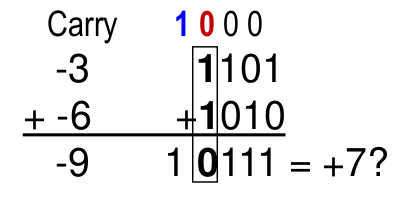
\includegraphics[width=0.3\linewidth]{ex3}
			\end{center}
			Here overflow occurs since the bit into carry 0 is not the same as the bit out of carry 1. 
		
		\end{mdframed}
		
		\subsection{IEEE Floating Point}
		This is a standerdized way of representing floating bit numbers. 
		
		We have 3 parts to the 32 bit number to represent a binary number $n$. 
		\begin{enumerate}[]
			\item Sign (1 bit)
			\item Exponent (8 bits) - 127 + The exponent the fractional part needs to be raised to to get $n$ 
			\item Mantissa (23 bits) - The fractional part of the normalized number $n$
		\end{enumerate}
	
		\begin{mdframed}[]
		\textbf{Ex. Express $(36.5625)_{10}$ as a 32 bit FP number using the IEEE standard.}
		
		The value in binary is $100100.1001$ and normalized is $1.001001001 \times 2^5$.
		
		\begin{enumerate}[noitemsep]
			\item Sign: 0
			\item Exponent: 5+127 = 131 = 10000100 
			\item Mantissa: 00100100100000000000000
		\end{enumerate}
		
		So the 32 bit number is: 0 10000100 00100100100000000000000 (without the spaces ofc)
		\end{mdframed}
		
		\section{Chapter 4}
		
		An operation executed in \textit{one} clock cycle is called a \textbf{micro operation}.
		
		\subsection{Arithmetic Operations}
		These are things such as adding, subtracting, and really anything that uses an adder block.
		
		\subsection{Logic Operations}
		These are things that are not arithmetic but are still done such as AND, OR, SHIFTS, etc.
		
		A circular shift will shift everything left or right and the spare bit will be taken from the other side.
		
		A logical shift will shift everything left or right and the spare bit will be always a 0.
		
		An arithmetic shift will shift everything left or right and the spare bit if right will be the same as the original MSB, and if left will be 0.
		
		Right Arithmetic shift is division, and Left Arithmetic shift is multiplication.
		
		\section {Chapter 5}
		For this entire chapter (and course) we consider a computer to have 16 bits. So each instruction has 16 bits, and each register can hold at most 16 bits (some are less though).
		
			\subsection{Instruction Codes}
			Each instruction is a group of 16 bits that instruct the computer what to do. 
			
			An instruction is divided into the \textbf{opcode }(\textit{First 4 bits}) and the \textbf{address }(\textit{Last 12 bits})
			
			The CU receives the instruction from memory, interprets the \textbf{opcode}, then issues a sequence of control signals to some of the registers, and maybe the ALU. 
			\begin{center}
				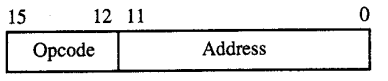
\includegraphics[width=0.3\linewidth]{opcode}
			\end{center}
			
			
				\subsubsection{MRI}
				Memory Reference Instructions (MRI) specify a \textbf{memory location using bits 0-11}. 
				
				For example, ADD \_\_\_ adds the content of the accumulator to the specified memory location. 
				
				\subsubsection{RRI}
				Register Reference Instructions (RRI) start with a 7 using bits 12-15, and then for bits 0-11, it uses those to also choose the instruction rather than a memory location.
				
				For example CMA will complement the accumulator, it uses\textbf{ no external memory address}, just the accumulator.
				
				\subsubsection{IOI}
				Input Output Instructions (IOI) work similar to RRI, but these are for input and outputs. 
			
			\subsection{Registers and BUS}
			The computer has the following registers:
			
			\begin{itemize}[noitemsep]
				\item AR: Address Register stores the memory address from bits 0-11 of the instruction
				\item PC: Program Counter stores the memory address of the next instructions
				\item DR: Data Register stores some data we want to use with the ALU
				\item AC: Accumulator which is the main register since it is the output of the ALU
				\item IR: Stores the current instruction code
				\item TR: Temporary Register is sometimes used for temporary storage
				\item OUTR/INPR: Holds Input or Output character.
			\end{itemize}
			
			\begin{center}
				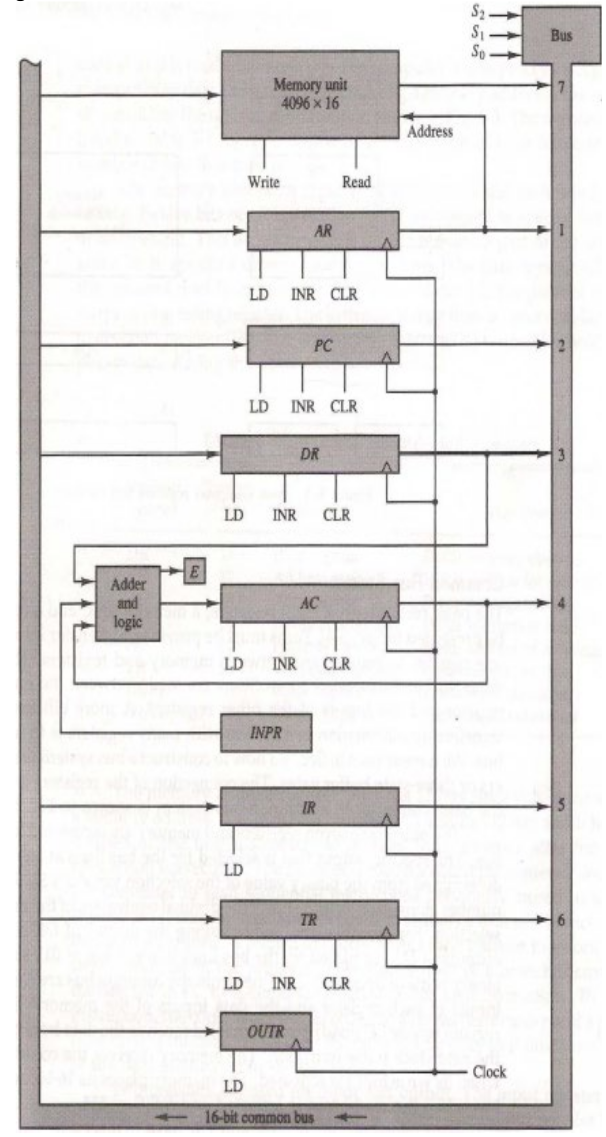
\includegraphics[width=0.4\linewidth]{registers}
			\end{center}
		
			Most of these registers can connect to the bus assuming the bus has that register selected. 
			
			\begin{mdframed}[]
			\textbf{Ex. } What is the state of the computer to send data from memory location 100 (in AR) to the DR?
			
			First we need to get the information into the bus. To do this, we need to set S2, S1, S0 to be 7, so 111. 
			
			The memory will read from the AR \textit{only if READ=1}, so we set READ to 1. 
			
			Now we load the DR (set LD of DR to 1).
			
			If we wanted, next cycle we could get it into the AC
			
			\end{mdframed}
			
			\subsection{Direct vs Indirect}
			If we say M[100], this means get the data located \textbf{in memory at location 100}. This is direct. 
			
			If we say M[M[100]], this means go to memory at location 100, and there will be a memory address. We want the \textbf{data at the memory address located at M[100]}. This is indirect.
			
			\subsection{Basic Computer Instructions}
			We have the following instruction list for the basic computer. 
			
			The first part are MRI, the second part RRI, the third part IOI.

			Note that I refers to indirect (1) or direct (0). 
			\begin{center}
				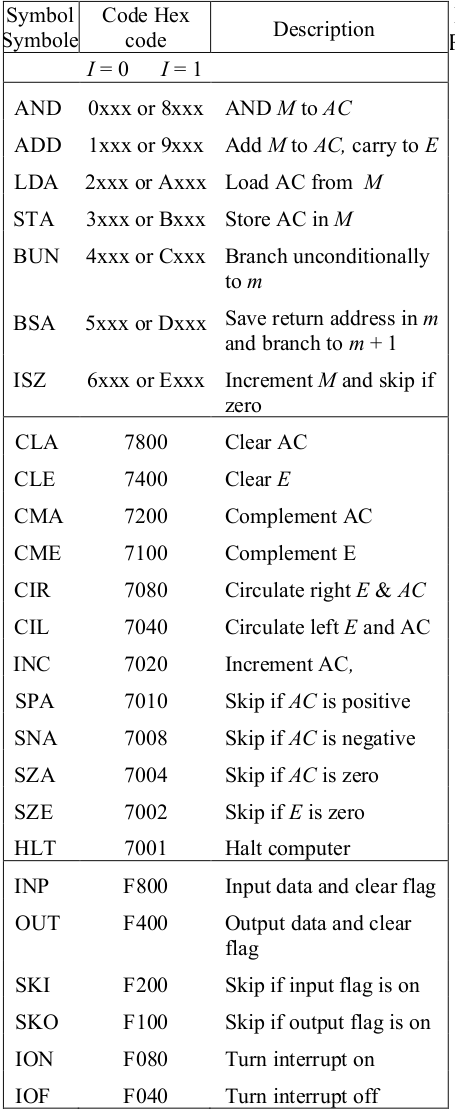
\includegraphics[width=0.4\linewidth]{instructions}
			\end{center}
			
			
				\subsubsection{ISZ}
				ISZ \_\_\_ will increment the memory location by 1, and then if it is 0, it will skip the next instruction.
				
				\subsubsection{BSA/BUN}
				BUN \_\_\_ will set the PC to the given memory location.
				
				BSA \_\_\_ will set the PC to the given memory location and save the current PC to memory location 0.
			
			\subsection{Timing}
			For timing stuff, we are working inside of the CU.
			
			Note that the CU works off of lots of binary bits such as\textbf{ T0-T15 (timing states), D0-7 (decoded opcode), IR0-IR11 (address of instruction)} and it outputs all the control signals for the bus, and registers (such as \textbf{DR Load, Memory READ}).
			
			We have a state counter (SC) which has 16 states and starts at 0, and each clock cycle increments. 
			
			\begin{center}
				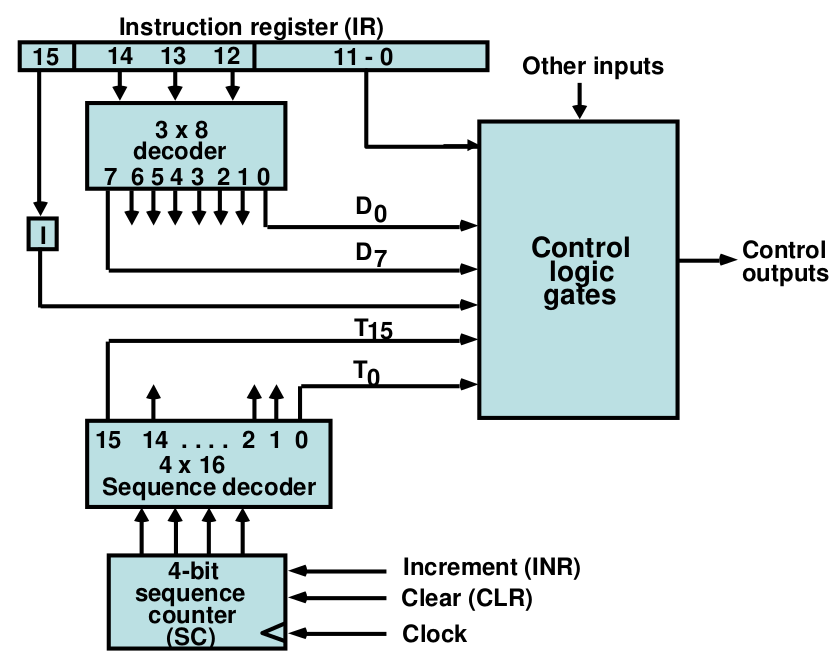
\includegraphics[width=0.6\linewidth]{cu}
			\end{center}
		
			The instruction cycle has the following 4 phases:
			\begin{enumerate}[]
				\item Fetch instruction from memory T0, T1
				\item Decode the instruction T2
				\item Read the address from memory if indirect address
				\item Execute the instruction
			\end{enumerate}
		
			We have the following instruction cycle. 
			
			\begin{center}
				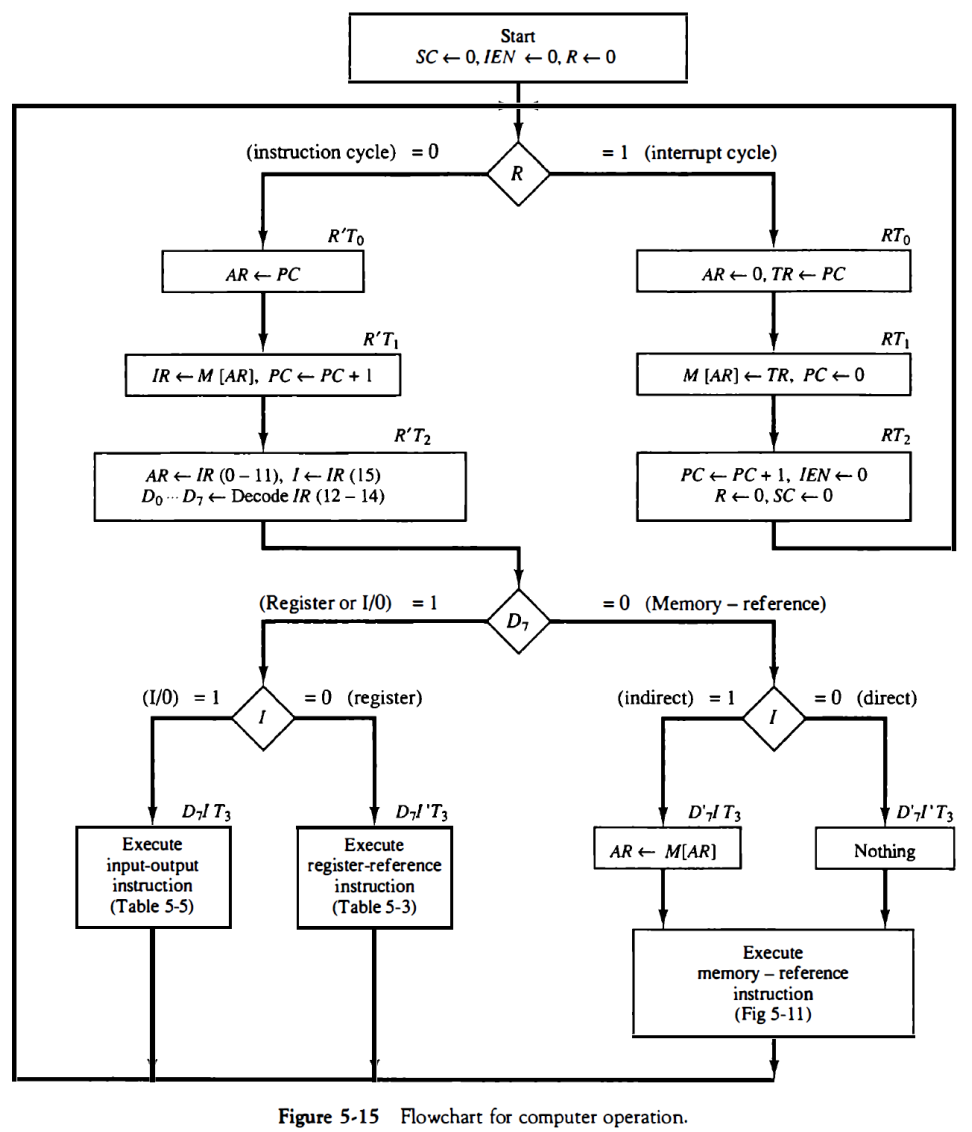
\includegraphics[width=0.7\linewidth]{instruction_cycle}
			\end{center}
		
			Note how at the bottom of each column, it says "execute the instruction". We have a table with the exact instructions for each of these operations, or we can come up with it logically. 
			
			\begin{center}
				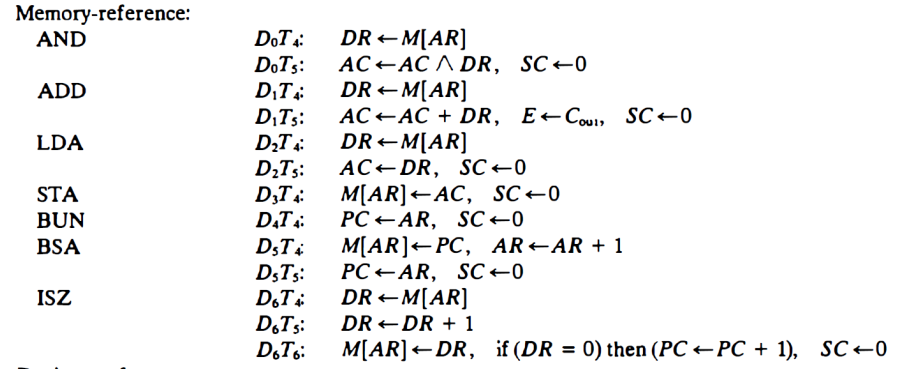
\includegraphics[width=0.7\linewidth]{instructionsss}
			\end{center}
		
			We also have one for RRI and IOI.
			
			\subsection{Interrupt}
			The ION and IOF instructions will enable and disable the interrupt (IEN register) respectively. 
			
			When the interrupt is on (IEN=1), we use a \textbf{flag} called R (just a flip flop).
			
			R is checked at the\textbf{ start of each instruction cycle}. If it is 1, then we branch to M[0] and execute the \textbf{interrupt sequence} stored there. 
		
		
		
		
		\section{Chapter 6}
		Machine language is a sequence of commands representing the exact content in memory. 
		
		Assembly is like machine language but there are comments, and variables. 
		
			\subsection{Assembly Syntax}
			In assembly, we have 3 columns.
			
			\begin{tabular}{|c|c|c|}
				\hline
				Label & Instruction & Comment \\
				\hline
				Optional & Mandatory & Optional \\
				\hline
			\end{tabular}
		
			\begin{mdframed}[]
				This is an example of assembly code with comments
			\begin{lstlisting}
     ORG 100 /sets origin of program (here) to 100
     LDA HEX A2 /loads hex value A2 into AC
CTR, DEC -2 /creates counter variable with decimal value -2
LOP, ISZ CTR /increments CTR, skips next line if 0 (will be -1)
     BUN LOP /branches to the line with LOP (the ISZ)
     HLT /halts the computer				
			\end{lstlisting}
				This code will loop twice before getting 0 in CTR, then it will skip the BUN line, and HLT the computer.
			\end{mdframed}
		
			The \textit{label }can be a string up to 3 letters, that cannot start with a number. 
			
			The \textit{instruction} can be any RRI, MRI, or IOI instruction, or a psudocode (ORG, END, DEC, HEX).
			
			To use \textbf{indirect addressing}, we put an I at the end of the instruction.
			\begin{mdframed}[]
				\begin{lstlisting}
ORG 100 /sets origin of program (here) to 100
LDA x I /loads M[M[x]]
x, HEX 111	
END				
				\end{lstlisting}
			\end{mdframed}
			
			\subsection{Assembler}
			The assembler converts assembly to binary that the computer can handle. 
			
			The first pass generates the address symbol table which maps the variables to their binary equivalent. 
			
			The second pass translates everything else to binary.
			
			\subsection{Double Precision}
			When we want to add 2 numbers which have double precision (2 memory locations for each number), we need to be careful.
			
			\begin{enumerate}
				\item Add the lower halves together
				\item Save result
				\item Get the carry from E into AC (using CLA, then CIL)
				\item Add both upper halves to the carry
				\item Save result 
			\end{enumerate}
			
			\subsection{Subroutines}
			A subroutine is called using the \textbf{BSA} instruction. We will BSA to the \textbf{address of the subroutine} (which \textit{saves the current address at the address of subroutine}), and then at the end of the subroutine, BUN back to the main code (BUN to \textit{start of subroutine} indirectly). 
			
			To pass data from the main to subroutine, we can either store it in a register, or/and store it after the BSA call. 
			
			\begin{mdframed}[]
			
			\begin{lstlisting}[]
    ORG 100
    BSA SUB /call subroutine
    HEX 123 /parameter passed into subroutine
    HLT /program done
SUB HEX 0 /start of subroutine, will store location to after BSA
    LDA SUB /since SUB now has HEX 123, loads that
    ISZ BSA /we do not want to return to 123, but to HLT
    BUN BSA /this returns to the HLT line

			\end{lstlisting}
			\end{mdframed}
		
		
		
		
		
		
		
	
	
	
	
\end{document}